\section{КОНСТРУКТОРСКИЙ РАЗДЕЛ}

В разделе описывается метод распознавания суицидальных паттернов поведения человека по текстовым сообщениям, а также формат и метод сбора задействованных в нем данных. 
Приводится диаграмма вариантов использования, декомпозиция задачи распознавания суицидального сообщения, а также диаграмма ``сущность-связь'' в нотации Чена. 
Определяется перечень задействованных методов машинного обучения и векторизации.

\subsection{Формат и метод сбора данных}

В качестве задействованных в анализе данных используются текстовые сообщения. 
Для сбора данных потребуется использовать автоматизированное средство сбора суицидальных сообщений в мессенджере Telegram. 
Интерфейс программного обеспечения позволяет направить в систему хранения два типа сообщений: суицидальные и на суицидальную тематику.

Средство сбора должно предоставлять пользователю следующий функционал:

\begin{enumerate}
\item[1.] Получение информации о проекте;
\item[2.] Получение информации об отличиях суицидальных сообщений и сообщений на суицидальную тематику;
\item[3.] Направление примеров суицидальных сообщений;
\item[4.] Направление примеров сообщений на суицидальную тематику, но не относящихся у суицидальным.
\end{enumerate}

Согласно 152-ФЗ ``О персональных данных'', ``персональные данные -- любая информация, относящаяся к прямо или косвенно определенному или определяемому физическому лицу (субъекту персональных данных)''~\cite{fzpers}. 
Таким образом, к персональным данным можно отнести фамилию, имя и отчество, дату и место рождения, адрес проживания, семейное, социальное и имущественное положение, образование, профессию, доходы и другое. 
В связи с этим средство сбора информации не обрабатывает и не хранит никаких персональных данных о пользователях, направивших сообщения.

\subsection{Средства реализации ботов в мессенджере Telegram}

В качестве представленных к использованию в качестве средства реализации бота в мессенджере телеграм могут быть задействованы популярные библиотеки:

\begin{itemize}
	\item Python Telegram Bot \cite{pythonTelegram},
	\item Telebot \cite{telebot},
	\item Node Telegram Bot API \cite{nodeTelegram},
	\item Telegram Bot Kotlin \cite{kotlinTelegram}.
\end{itemize}

Python Telegram Bot -- это библиотека, предоставляющая асинхронный интерфейс на ЯП Python для Telegram Bot API, которая совместима с версиями Python3.8 \cite{Python} и выше. 
Данная библиотека предоставляет высокий уровень абстракции и позволяет использовать объектно-ориентированный подход. 
Помимо реализации API, она также содержит ряд классов высокого уровня, упрощающих разработку ботов. 
Проект поддерживает строенную с асинхронным вводом-выводом.~\cite{pythonTelegram}

Telebot -- библиотека на Python, содержащая в себе асинхронную и синхронную реализацию Telegram Bot API. 
Данный проект предоставляет более гибкий и низкоуровневый доступ к API Telegram, чем упомянутый Python Telegram Bot.~\cite{telebot}

Node Telegram Bot API -- это библиотека для создания Telegram-ботов с использованием языка JavaScript~\cite{js} и платформы NodeJS~\cite{nodejs}. 
Несмотря на распространенное использование, используемая версия API Telegram является устаревшей.~\cite{nodeTelegram}

Telegram Bot Kotlin -- это библиотека для создания Telegram-ботов на ЯП Kotlin~\cite{Kotlin}. 
Отличительной особенностью является возможность разработки ботов на платформе Java Virtual Machine~\cite{jvm}, а также поддержка Kotlin Coroutines.~\cite{kotlinTelegram}

\subsection{Декомпозиция системы}

На рисунке \ref{img:useCase} представлена диаграмма вариантов использования системы.

\begin{figure}[H]
	\centering
	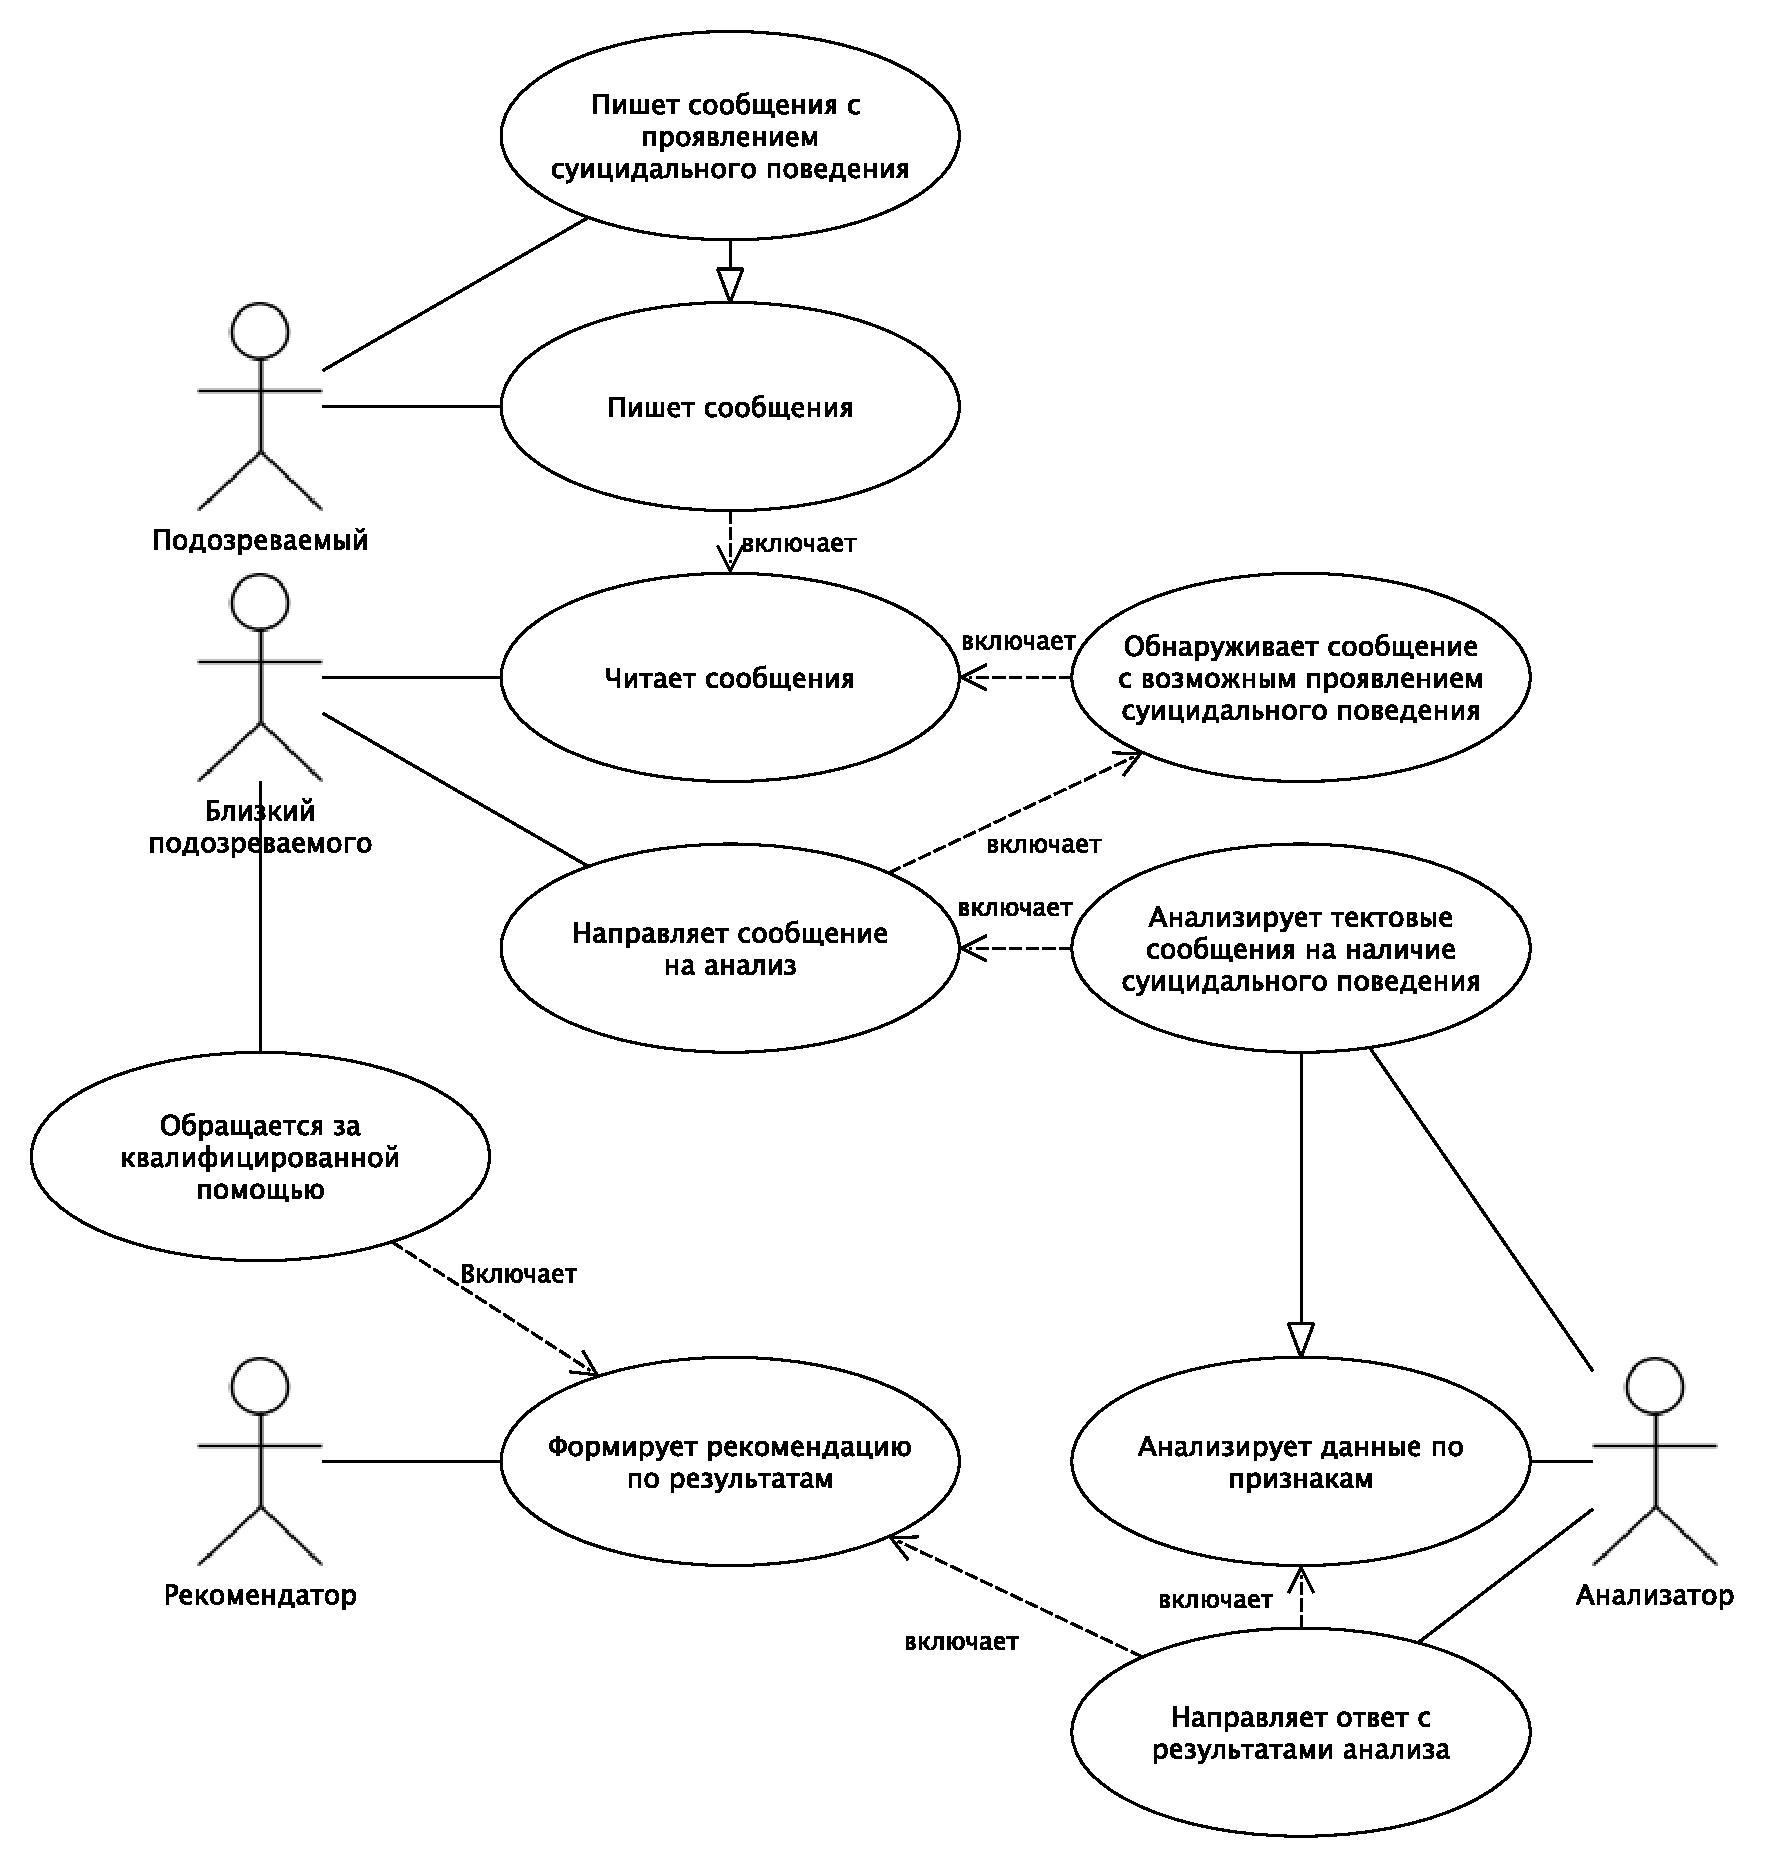
\includegraphics[width=\textwidth]{inc/useCase.pdf}
	\caption{ Диаграмма вариантов использования системы. }
	\label{img:useCase}
\end{figure}

На рисунке \ref{img:idef1} представлена IDEF0 диаграмма первого уровня задачи определения наличия суицидальных паттернов в текстовом сообщении.

\begin{figure}[H]
	\centering
	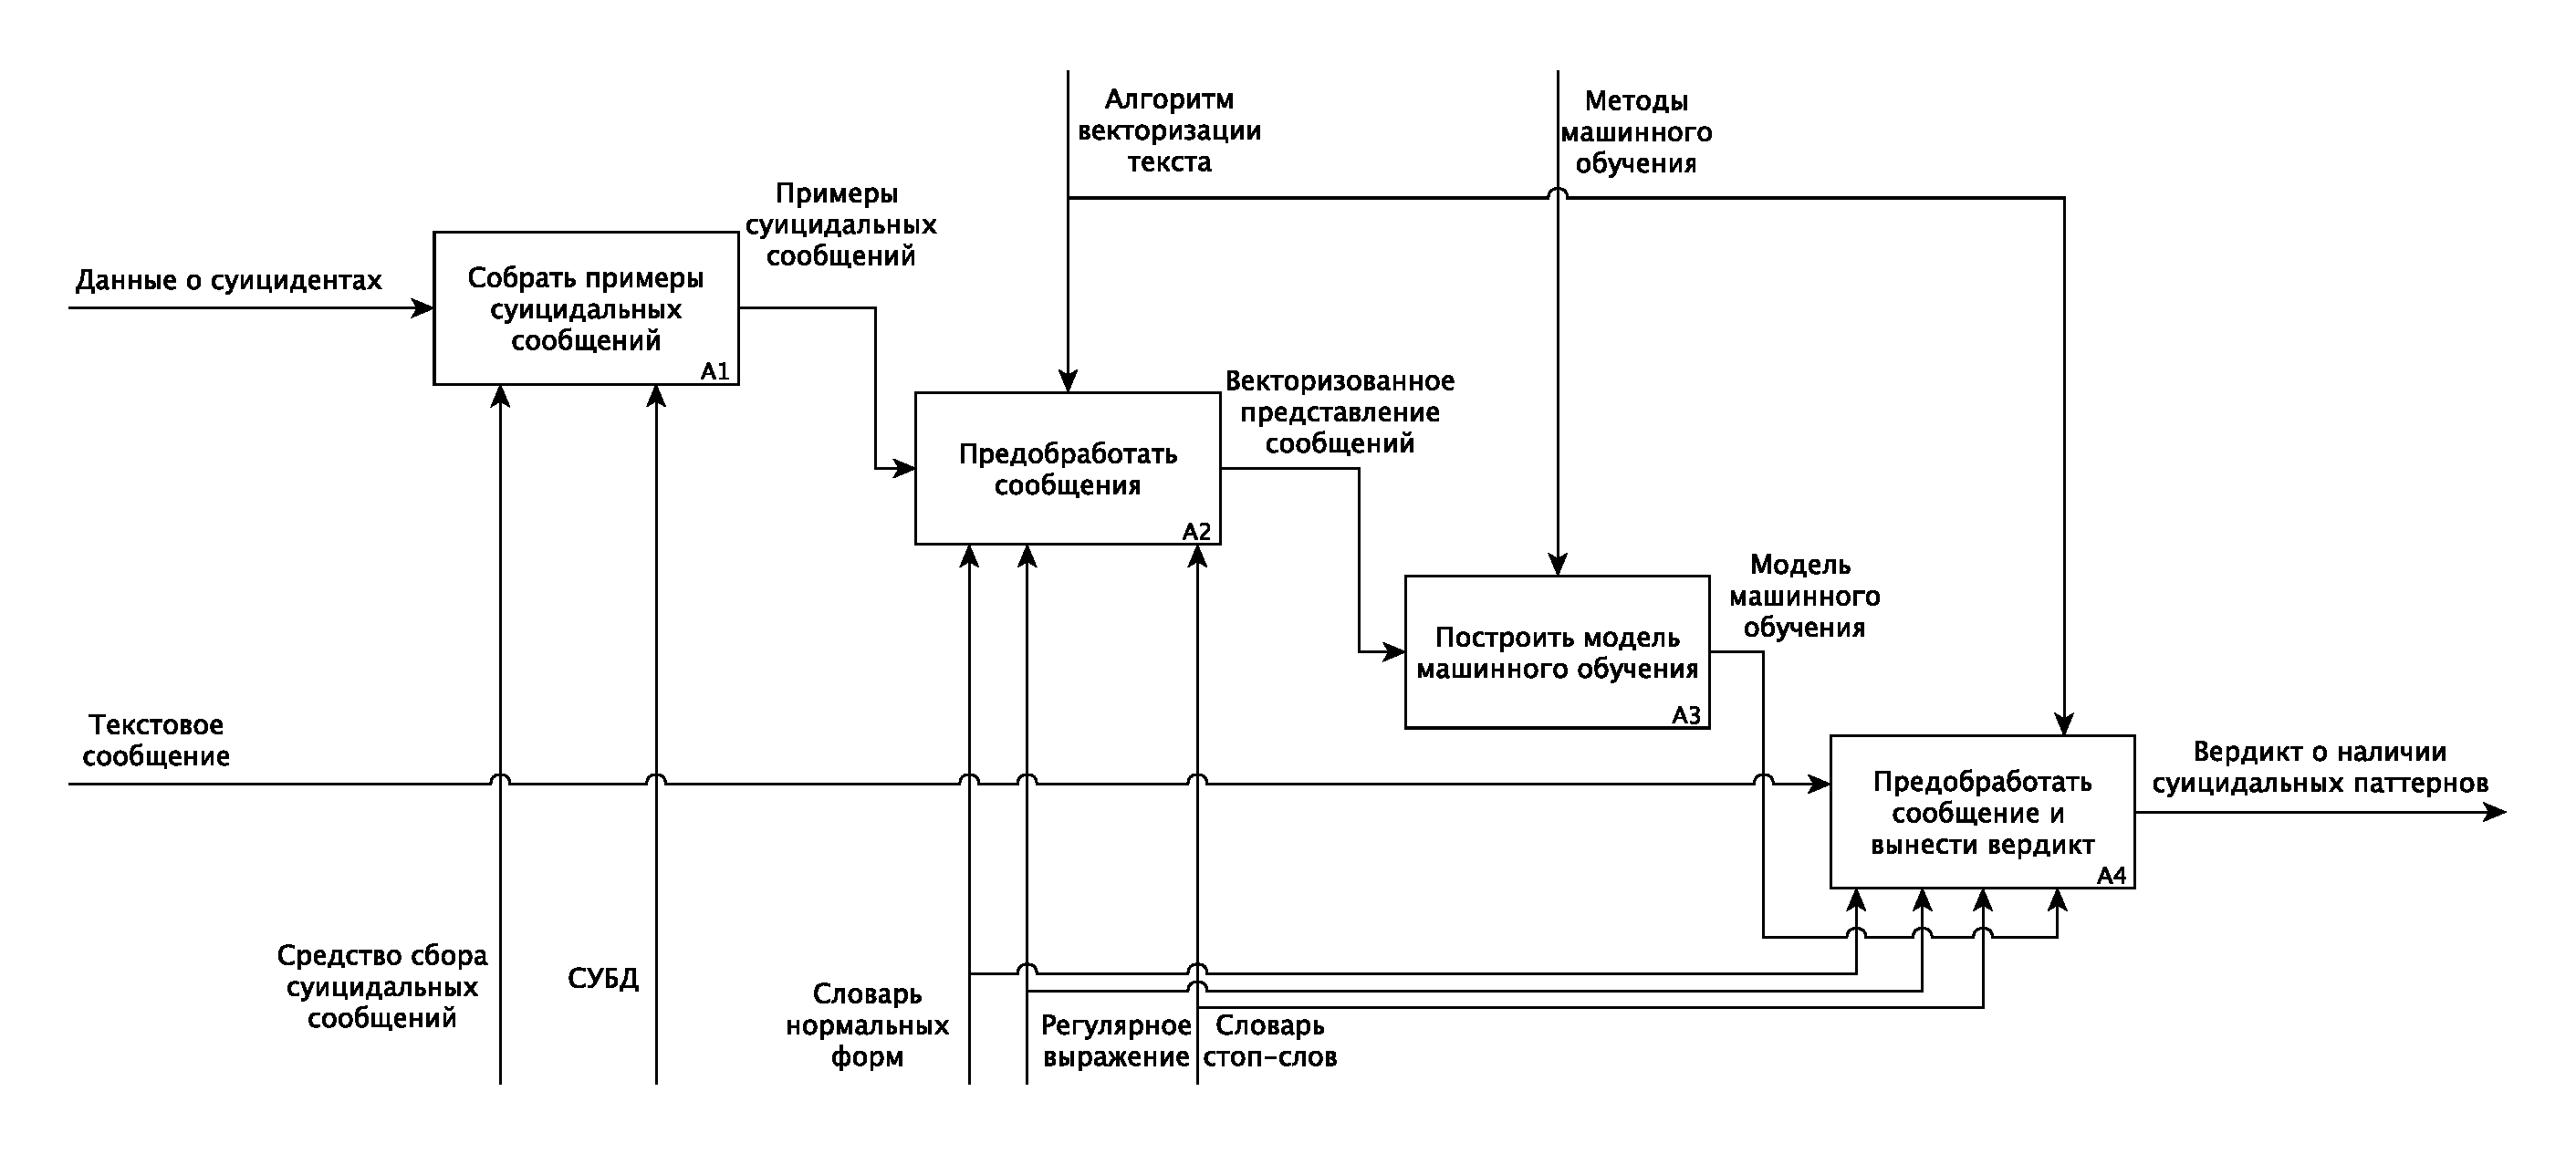
\includegraphics[width=\textwidth]{inc/A1.pdf}
	\caption{ IDEF0 диаграмма первого уровня. }
	\label{img:idef1}
\end{figure}

Модуль А1 на рисунке \ref{img:idef1} отвечает за сбор примеров суицидальных сообщений с использованием средства сбора суицидальных сообщений и СУБД. 
Средство сбора суицидальных сообщений в данном контексте подразумевает программное обеспечение, позволяющее пользователям вносить размеченные сообщения, то есть текст с указанным классом, к которому он относится. 
Затем эти данные будут задействованы в блоке предобработки сообщений.

Модуль А2 на рисунке \ref{img:idef1} отвечает за предобработку данных, собранных на этапах работы модуля А1. 
Данный блок включает в себя следующие шаги: токенизацию, лемматизацию, удаление стоп-слов и векторизацию.
В результате выполнения блока будет получено векторизованное представление поступивших в него примеров суицидальных сообщений, которое будет задействовано в дальнейшем в блоке построения модели машинного обучения.
Декомпозиция рассматриваемого блока приведена на рисунке \ref{img:idef21}.

\begin{figure}[H]
	\centering
	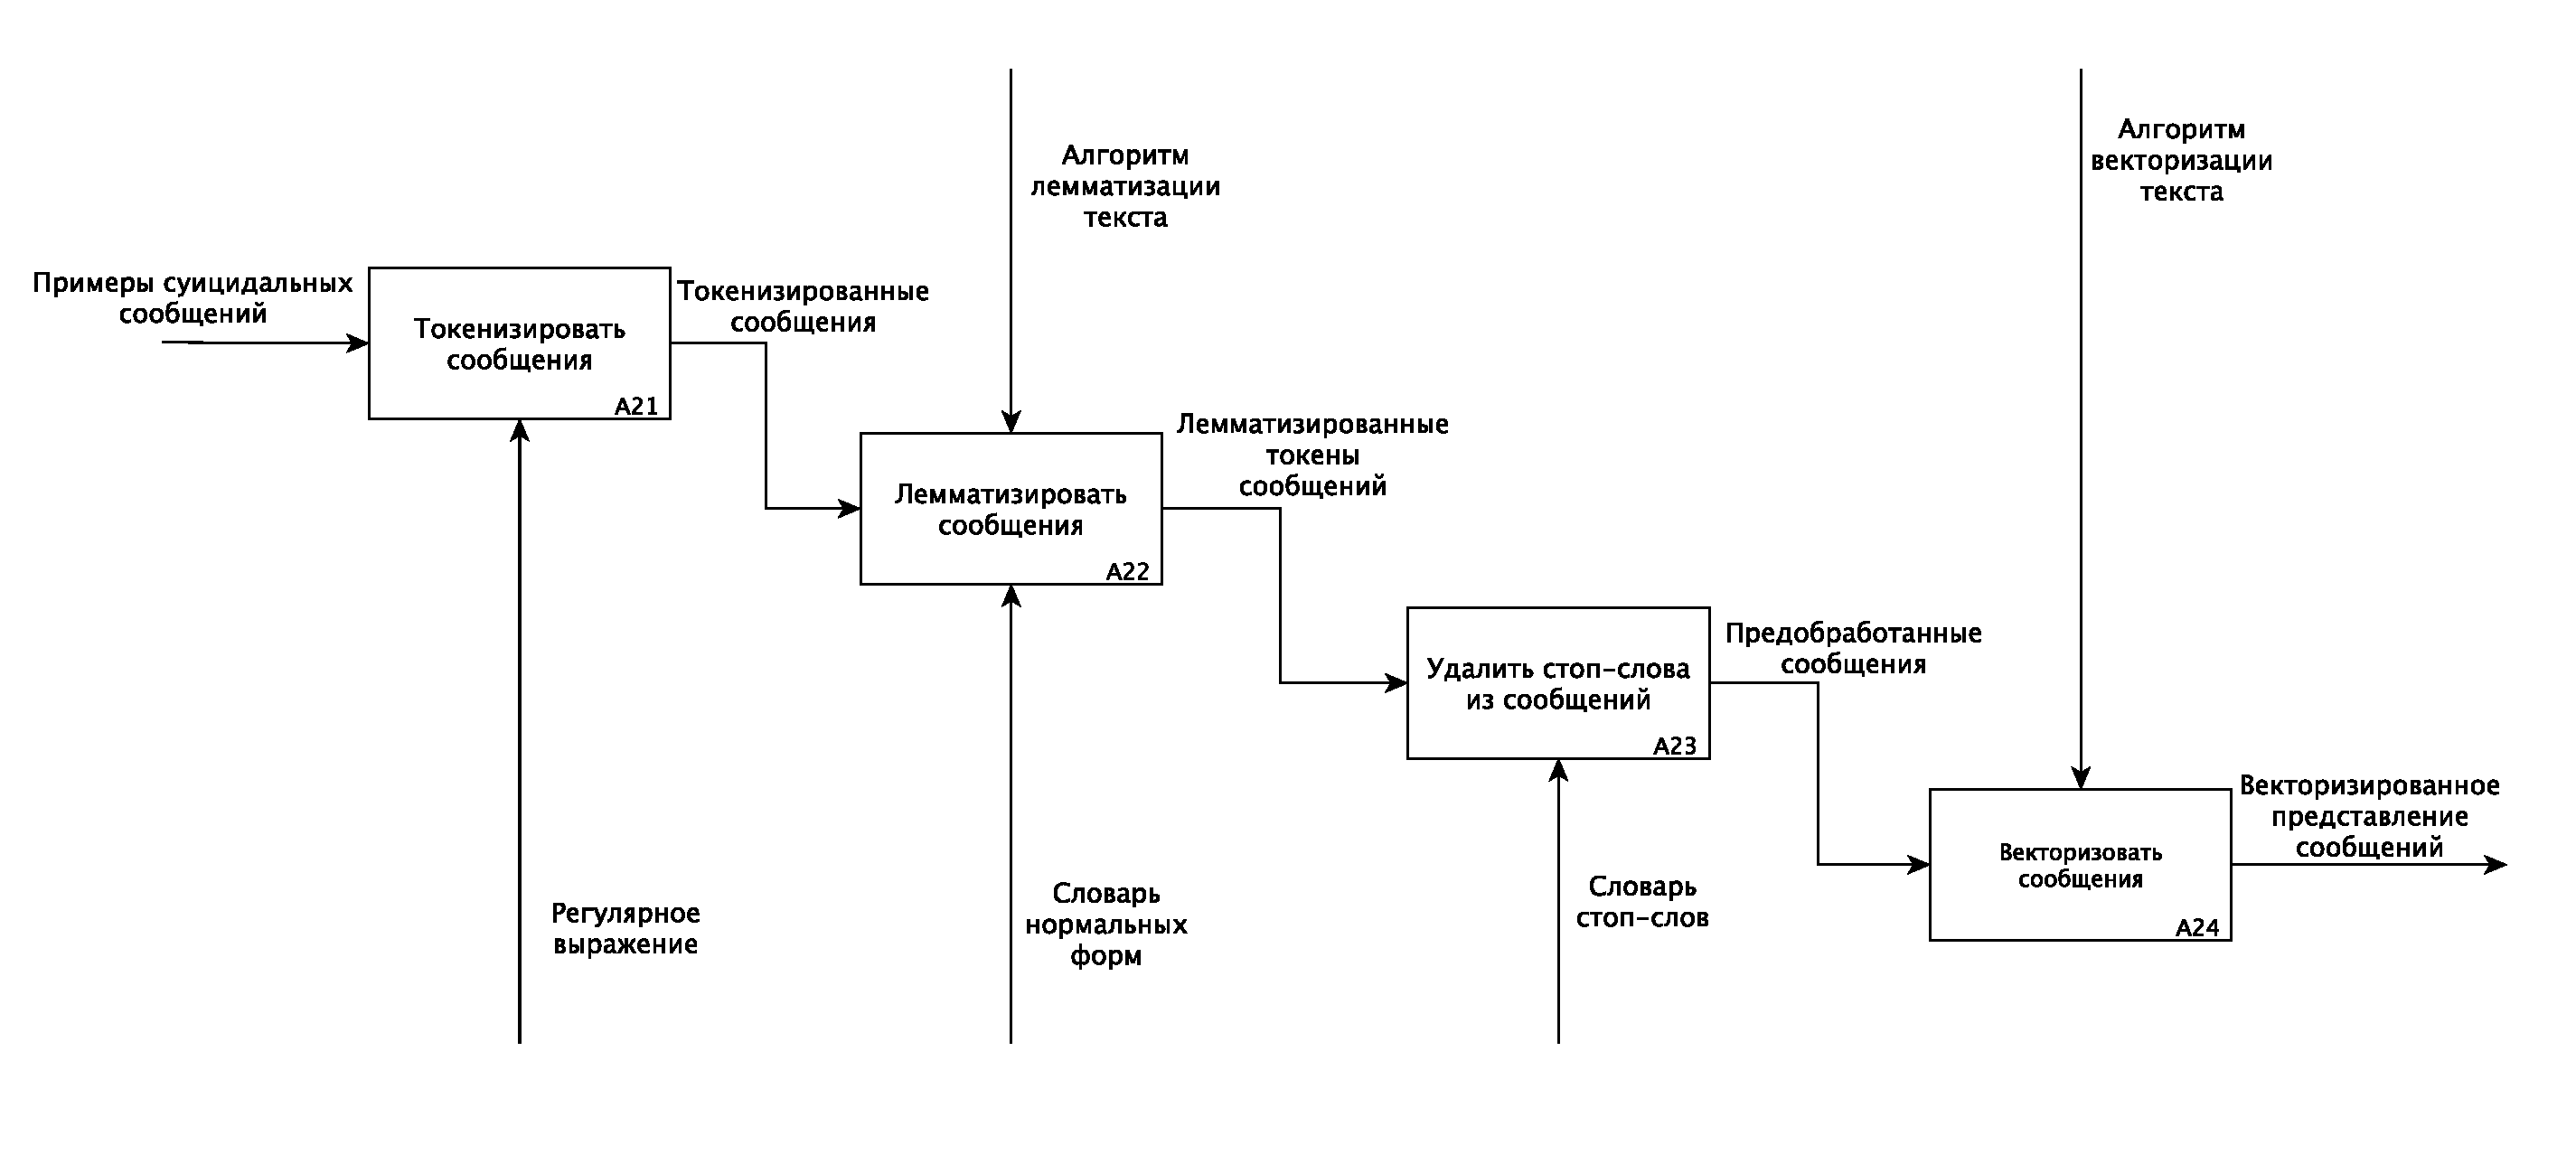
\includegraphics[width=\textwidth]{inc/A21.pdf}
	\caption{ IDEF0 диаграмма, декомпозиция блока A2. }
	\label{img:idef21}
\end{figure}

Модуль А3 на рисунке \ref{img:idef1} отвечает за построение модели машинного обучения, играющую роль классификатора сообщений. 
В качестве контроля блока выступают методы машинного обучения: градиентный бустинг, метод случайного леса, метод опорных векторов, метод К-ближайших соседей, логистическая регрессия и перцептрон.
В результате выполнения будет получена модель машинного обучения, задействованная в блоке предобработки поступившего вне обучающей выборки сообщения и вынесения вердикта о его суицидальности.

Модуль А4 на рисунке \ref{img:idef1} отвечает за предобработку поступившего в систему сообщения, а также его оценку на суицидальность. 
В качестве механизмов используются словарь нормальных форм, регулярное выражение и словарь стоп-слов для выполнения предобработки, а также модель машинного обучения для оценки сообщения.

На рисунке \ref{img:er} представлена диаграмма ``сущность-связь'' в нотации Чена.

\begin{figure}[H]
	\centering
	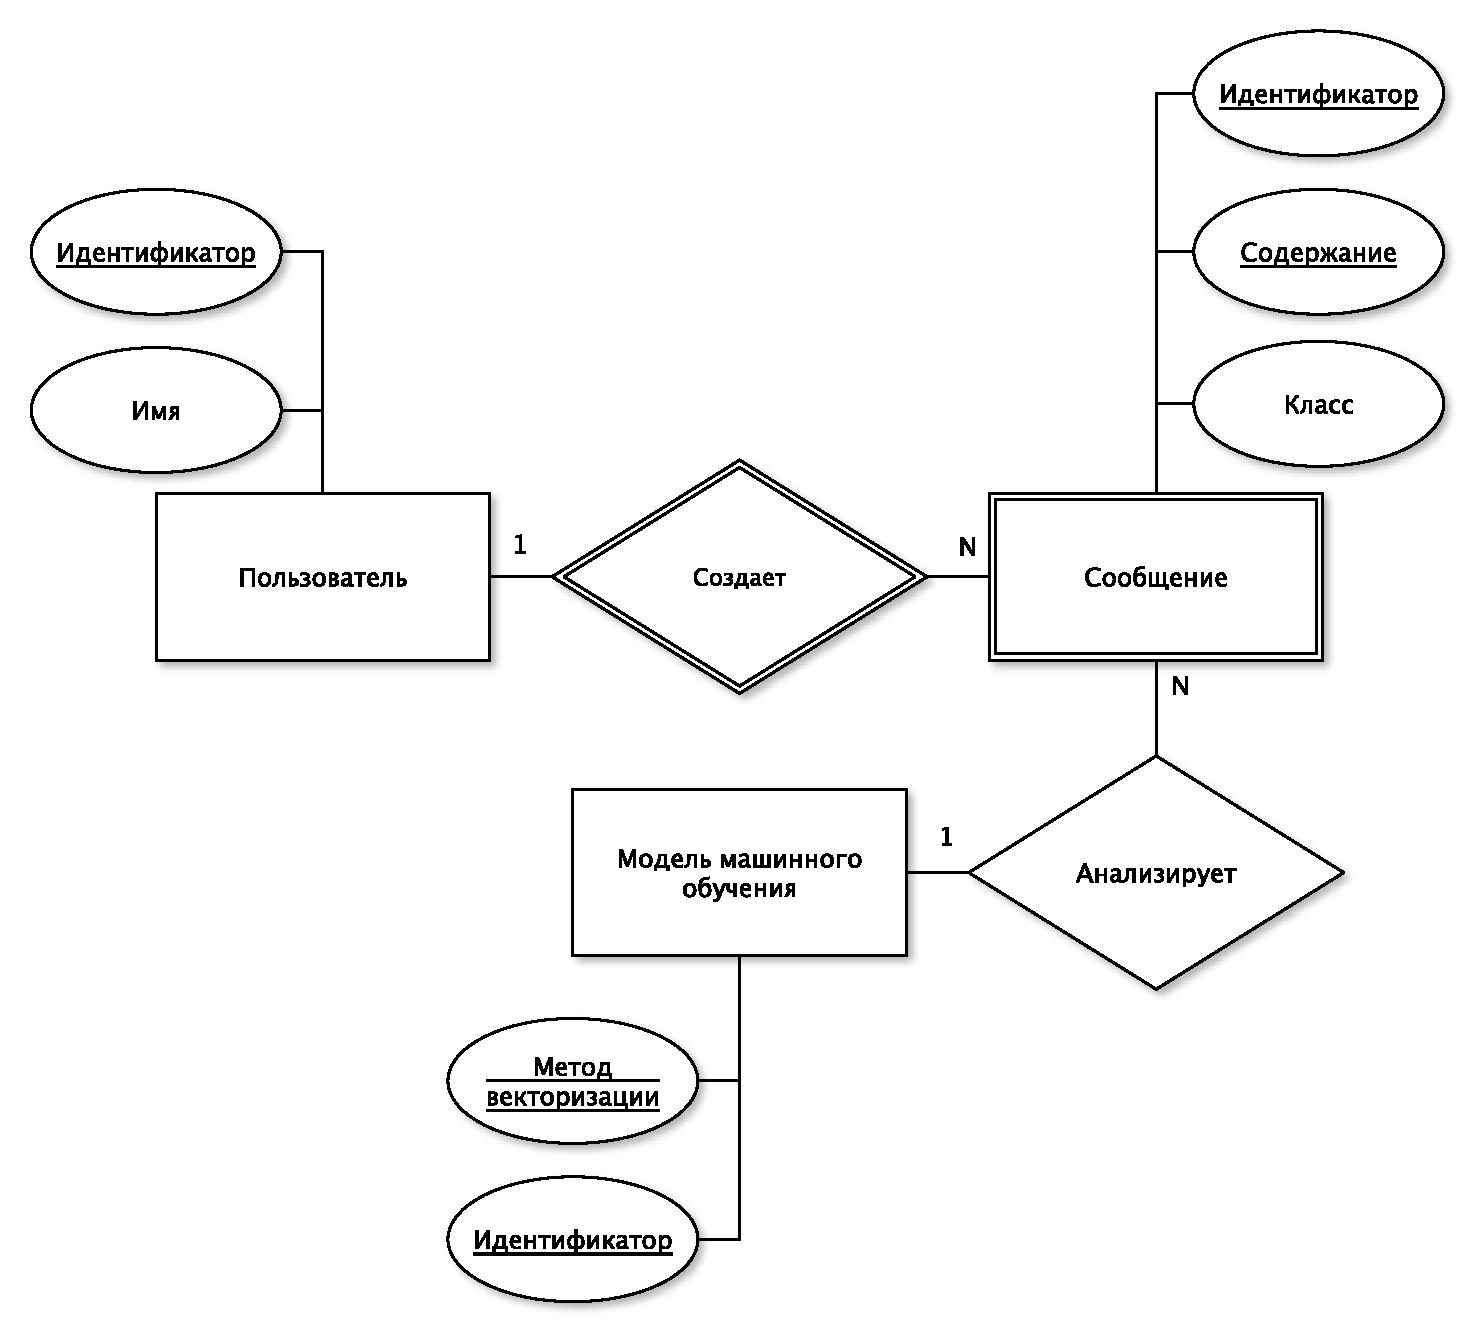
\includegraphics[width=0.7\textwidth]{inc/er.pdf}
	\caption{ Диаграмма ``сущность-связь'' в нотации Чена. }
	\label{img:er}
\end{figure}

На рисунке \ref{img:softScheme} представлена схема программного обеспечения.

\begin{figure}[H]
	\centering
	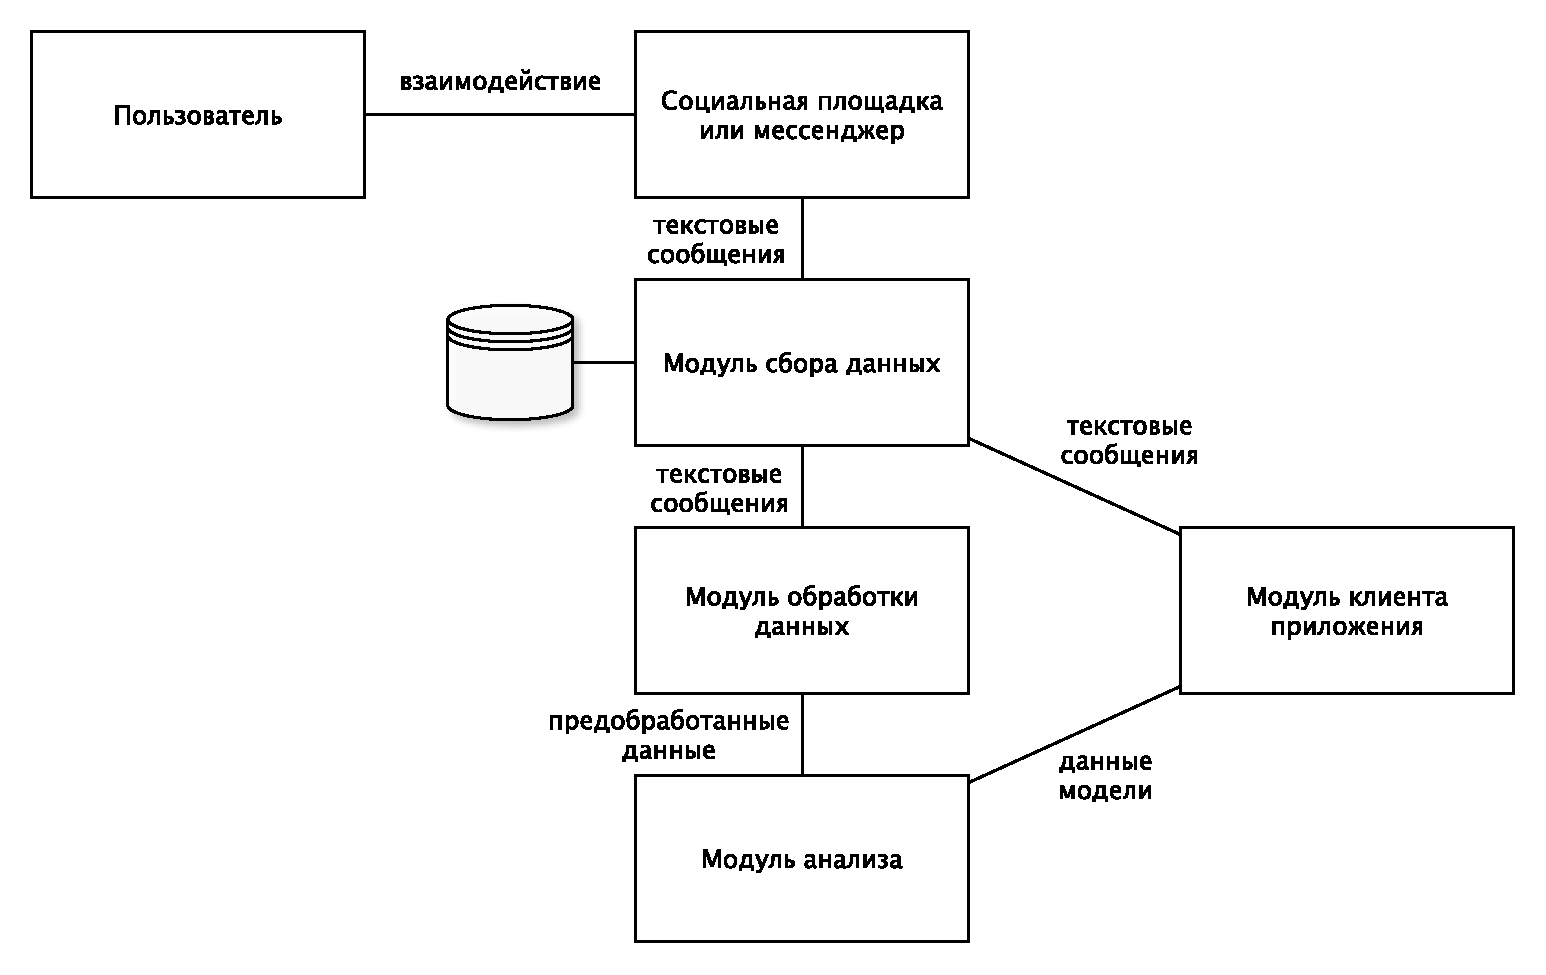
\includegraphics[width=0.9\textwidth]{inc/softScheme.pdf}
	\caption{ Схема программного обеспечения. }
	\label{img:softScheme}
\end{figure}


\subsection{Методы машинного обучения}

В качестве задействованных в методе алгоритмов рассматриваются: градиентный бустинг (схема алгоритма представлена на рисунке \ref{img:schemeGradient}), метод случайного леса (схема алгоритма представлена на рисунке \ref{img:schemeRandom}), метод опорных векторов (схема алгоритма представлена на рисунке \ref{img:schemeSvm}), метод К-ближайших соседей (схема алгоритма представлена на рисунке \ref{img:schemeKnn}), логистическая регрессия (схема алгоритма представлена на рисунке \ref{img:schemeLogistic}) и перцептрон (схема алгоритма представлена на рисунке \ref{img:schemePerceptrone}). Данный список обусловлен потребностью в целях исследования охватить широкий спектр методов машинного обучения для дальнейшего изучения возможности и потребности в создании ансамблевых моделей для решения поставленной задачи.

\begin{figure}[H]
	\centering
	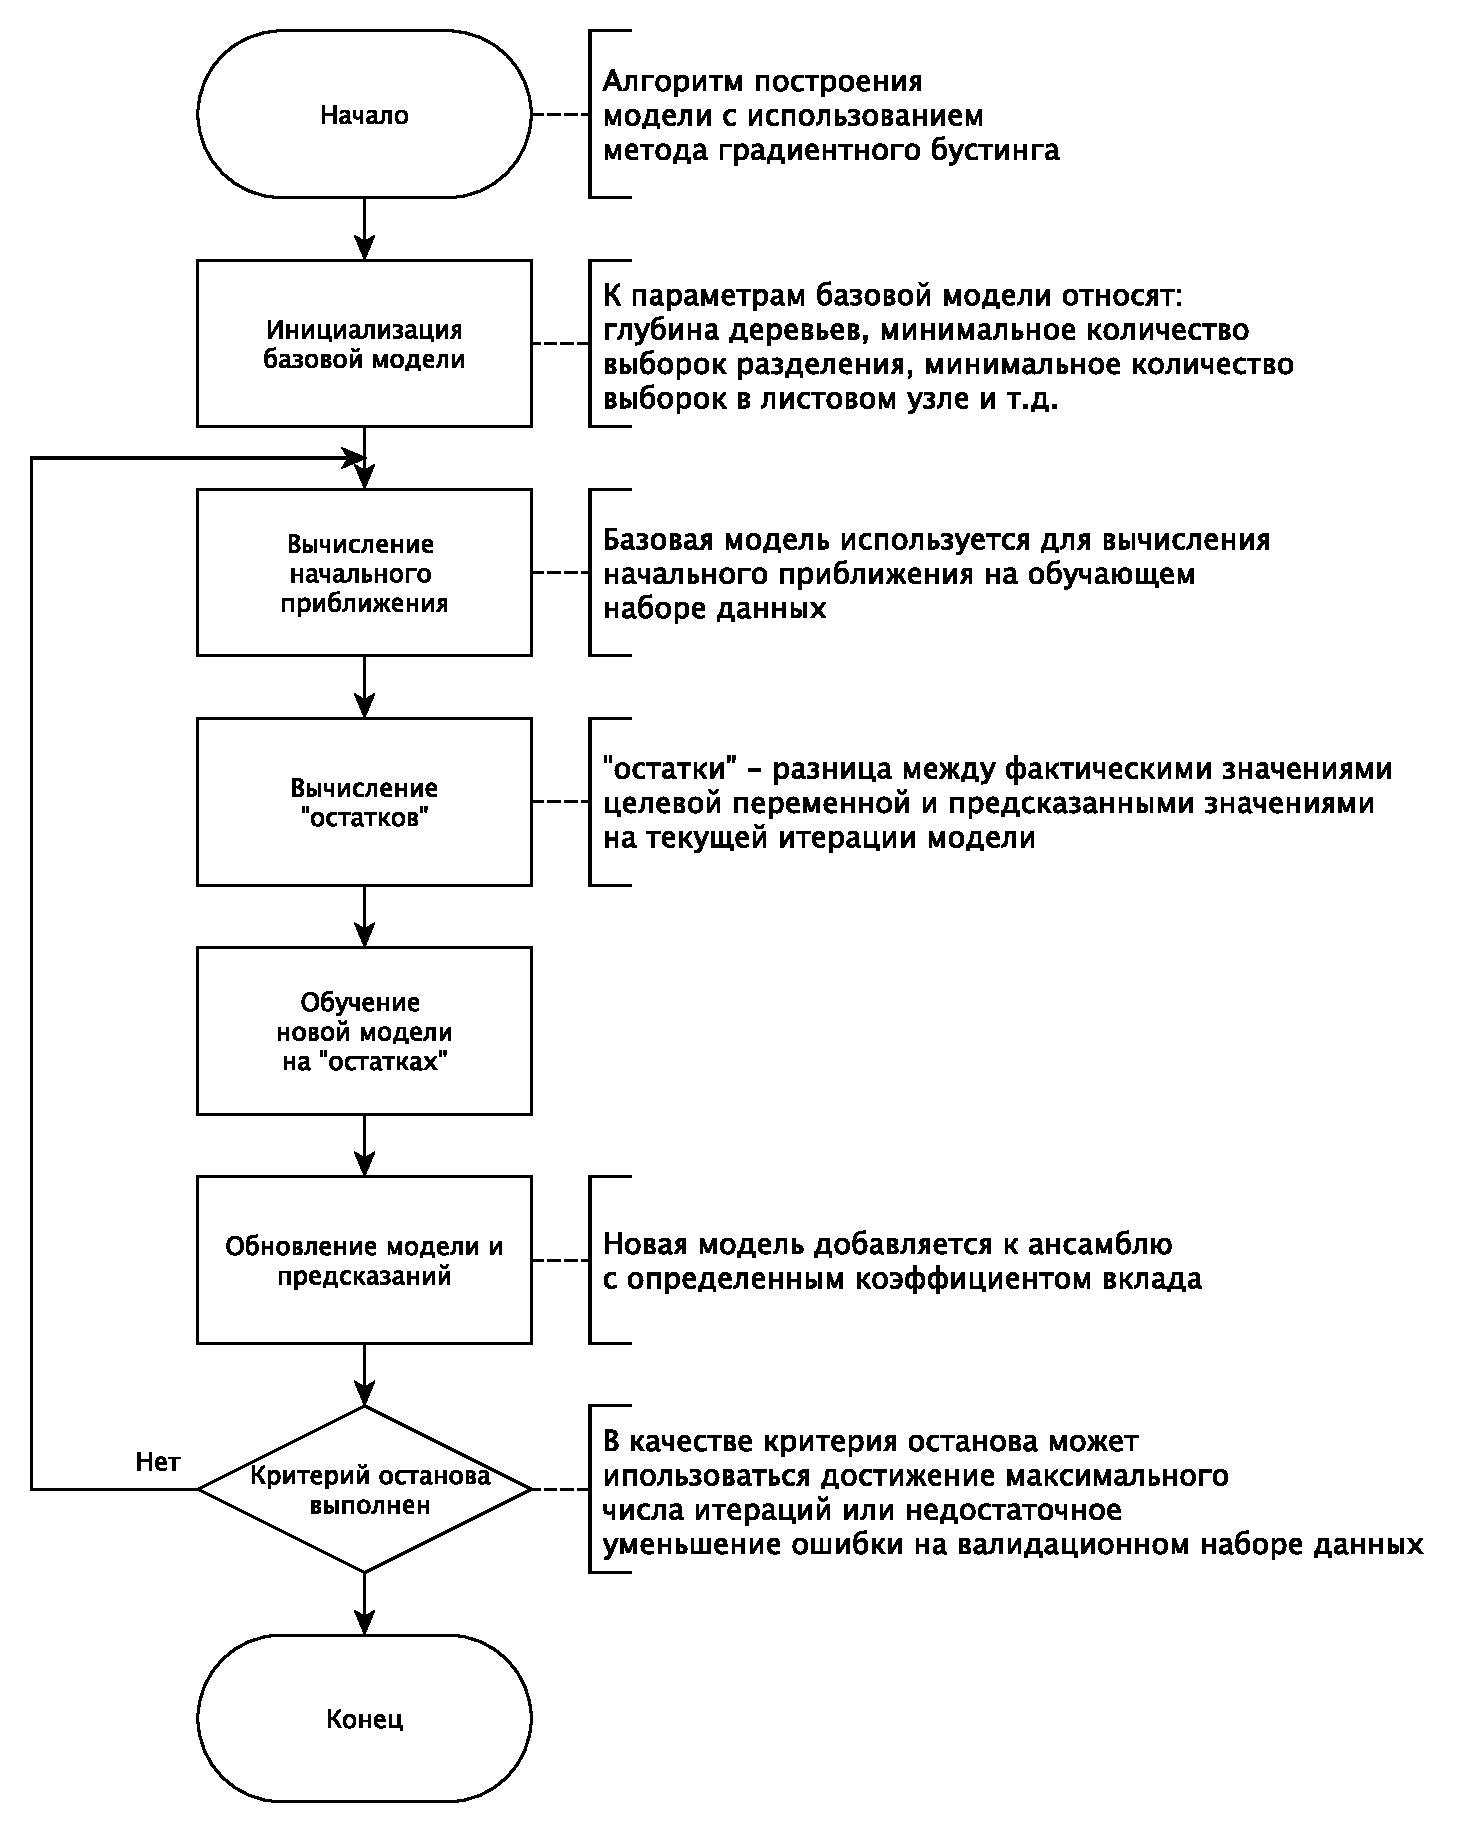
\includegraphics[width=\textwidth]{inc/schemeGradient.pdf}
	\caption{ Схема алгоритма работы градиентного бустинга. }
	\label{img:schemeGradient}
\end{figure}

\begin{figure}[H]
	\centering
	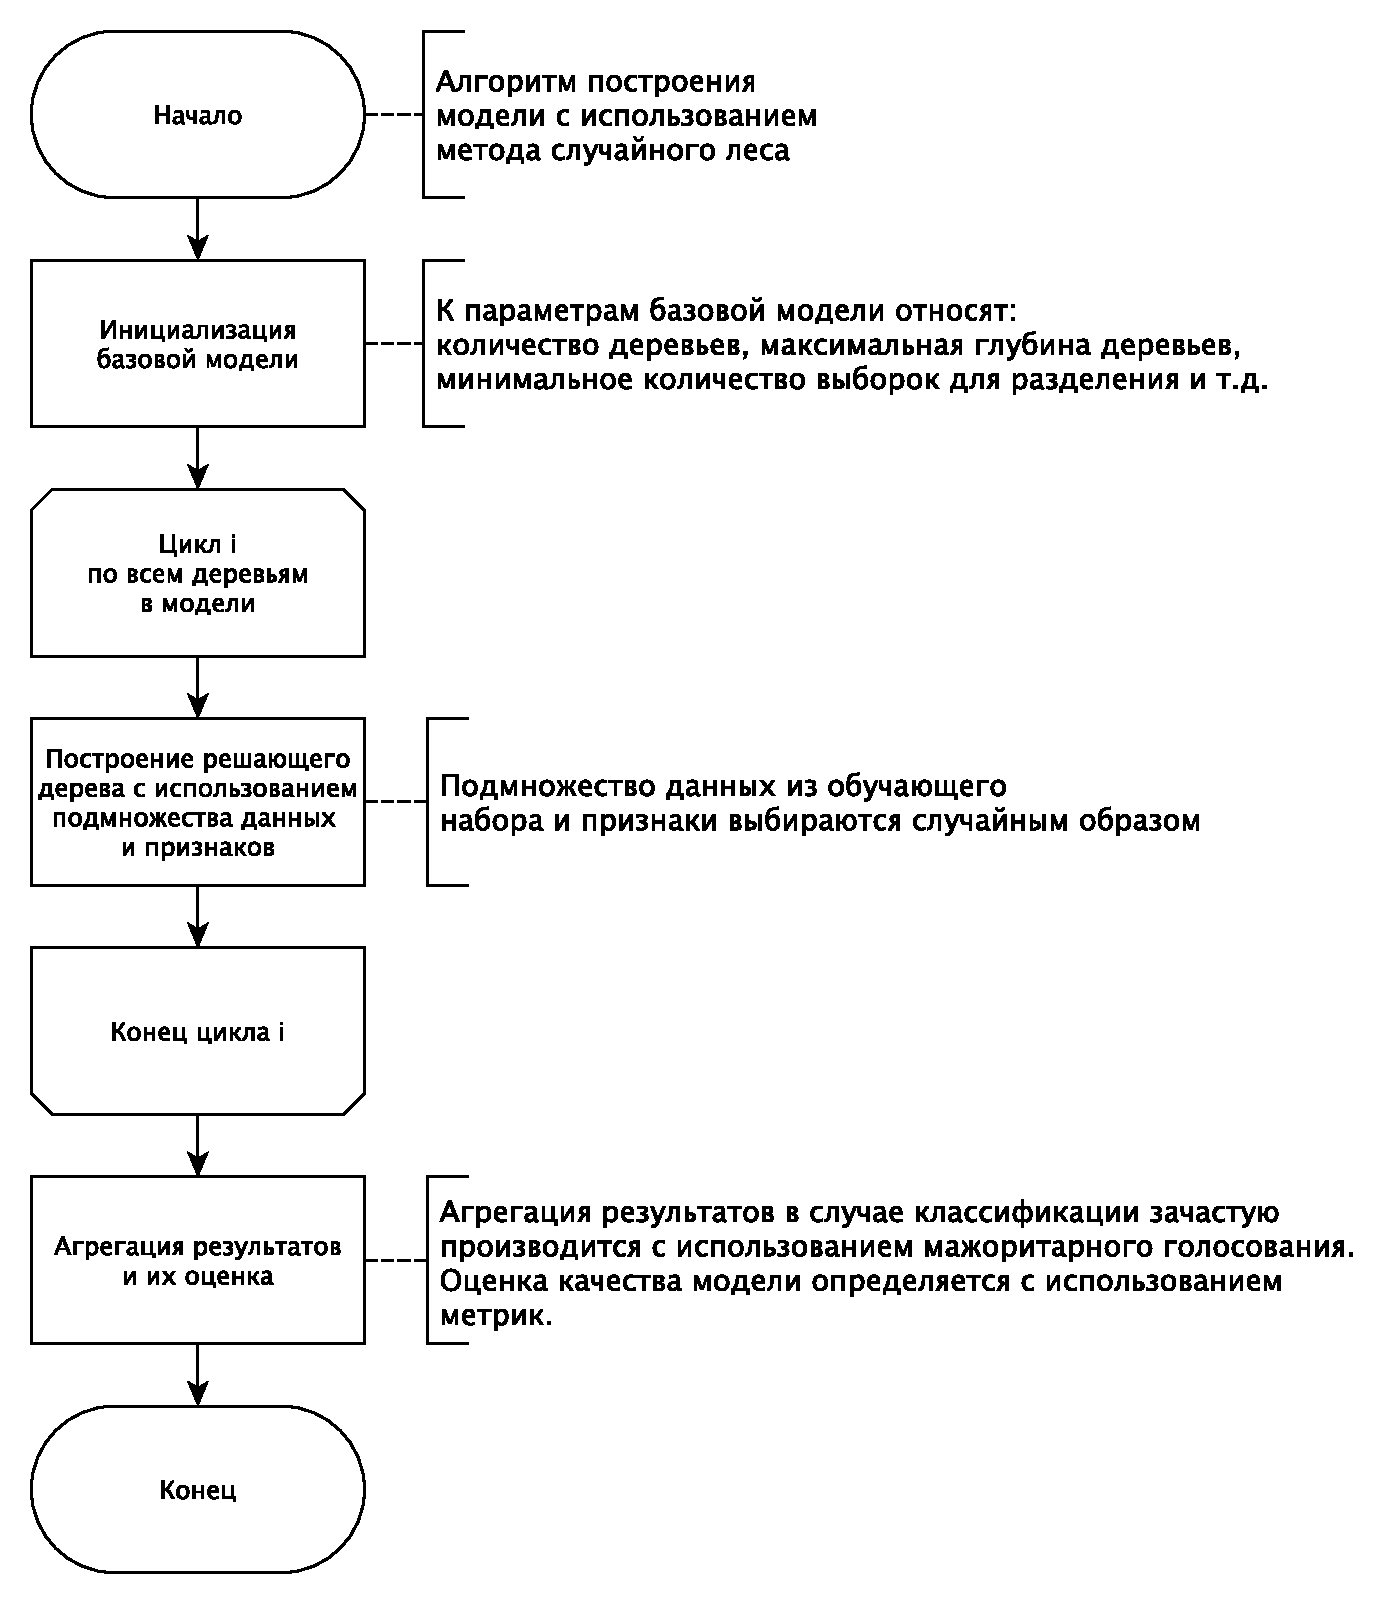
\includegraphics[width=\textwidth]{inc/schemeRandom.pdf}
	\caption{ Схема алгоритма работы метода случайного леса. }
	\label{img:schemeRandom}
\end{figure}

\begin{figure}[H]
	\centering
	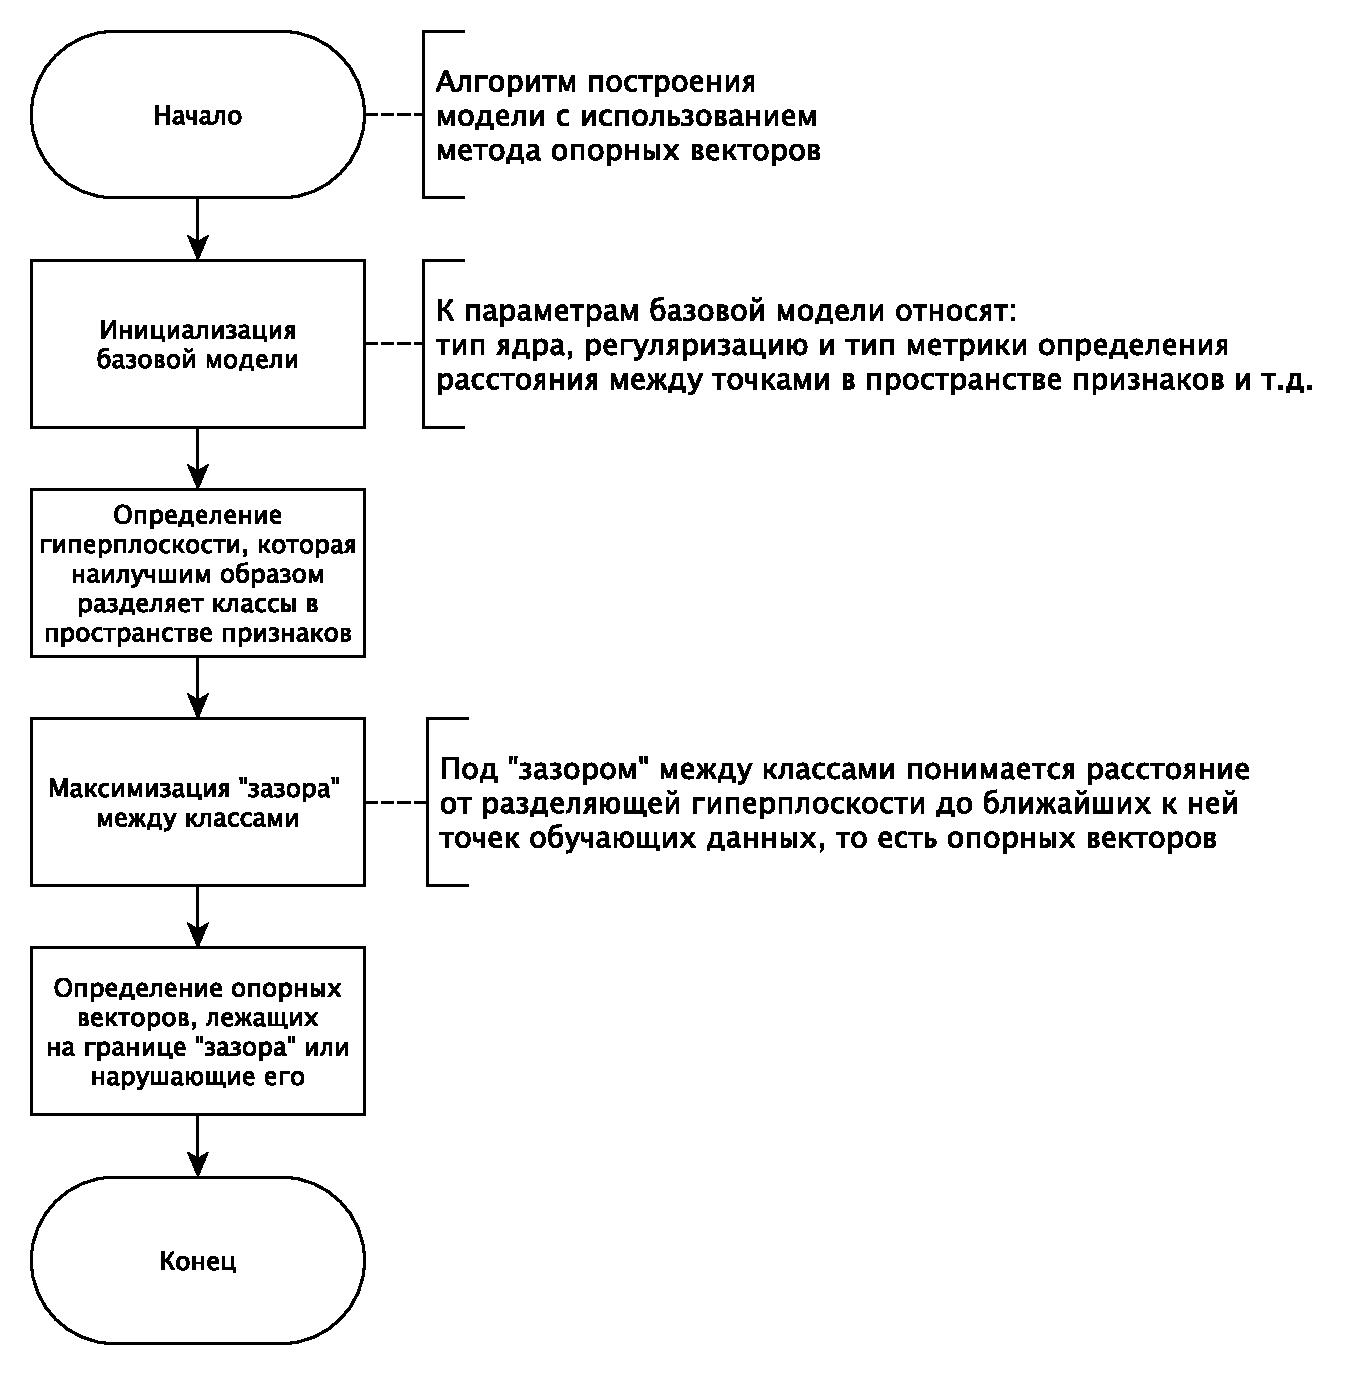
\includegraphics[width=0.7\textwidth]{inc/schemeSvm.pdf}
	\caption{ Схема алгоритма работы метода опорных векторов. }
	\label{img:schemeSvm}
\end{figure}

\begin{figure}[H]
	\centering
	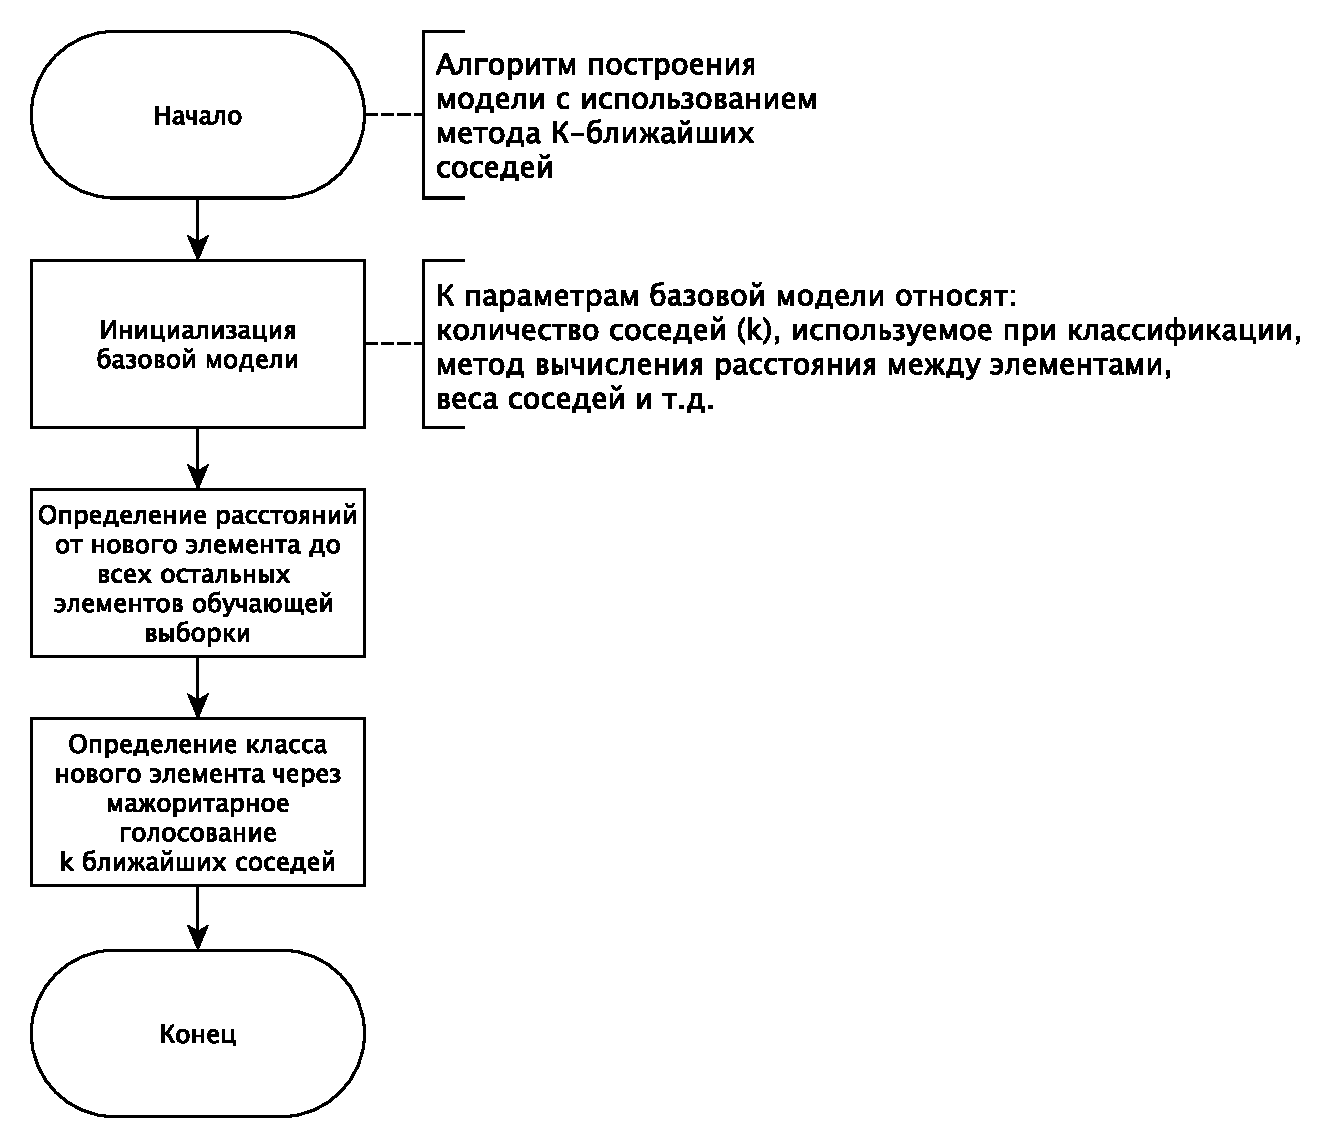
\includegraphics[width=0.7\textwidth]{inc/schemeKnn.pdf}
	\caption{ Схема алгоритма работы метода K-ближайших соседей. }
	\label{img:schemeKnn}
\end{figure}

\begin{figure}[H]
	\centering
	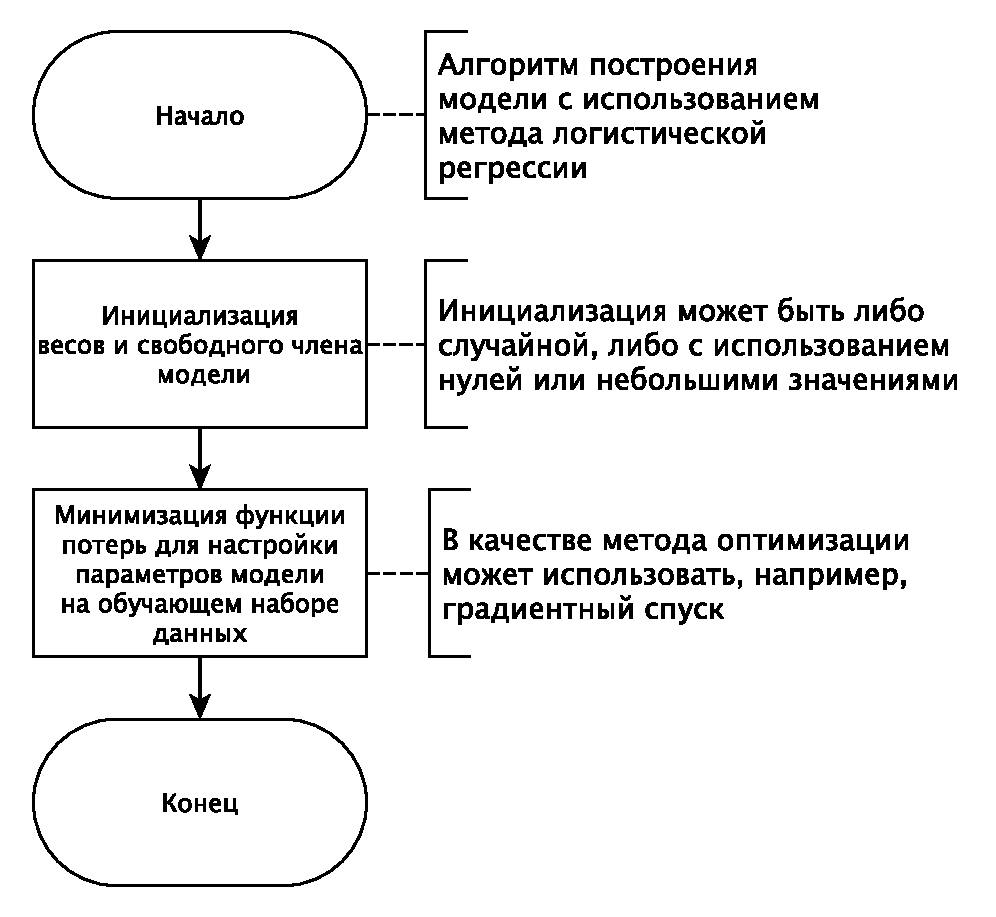
\includegraphics[width=0.7\textwidth]{inc/schemeLogistic.pdf}
	\caption{ Схема алгоритма логистической регрессии. }
	\label{img:schemeLogistic}
\end{figure}

\begin{figure}[H]
	\centering
	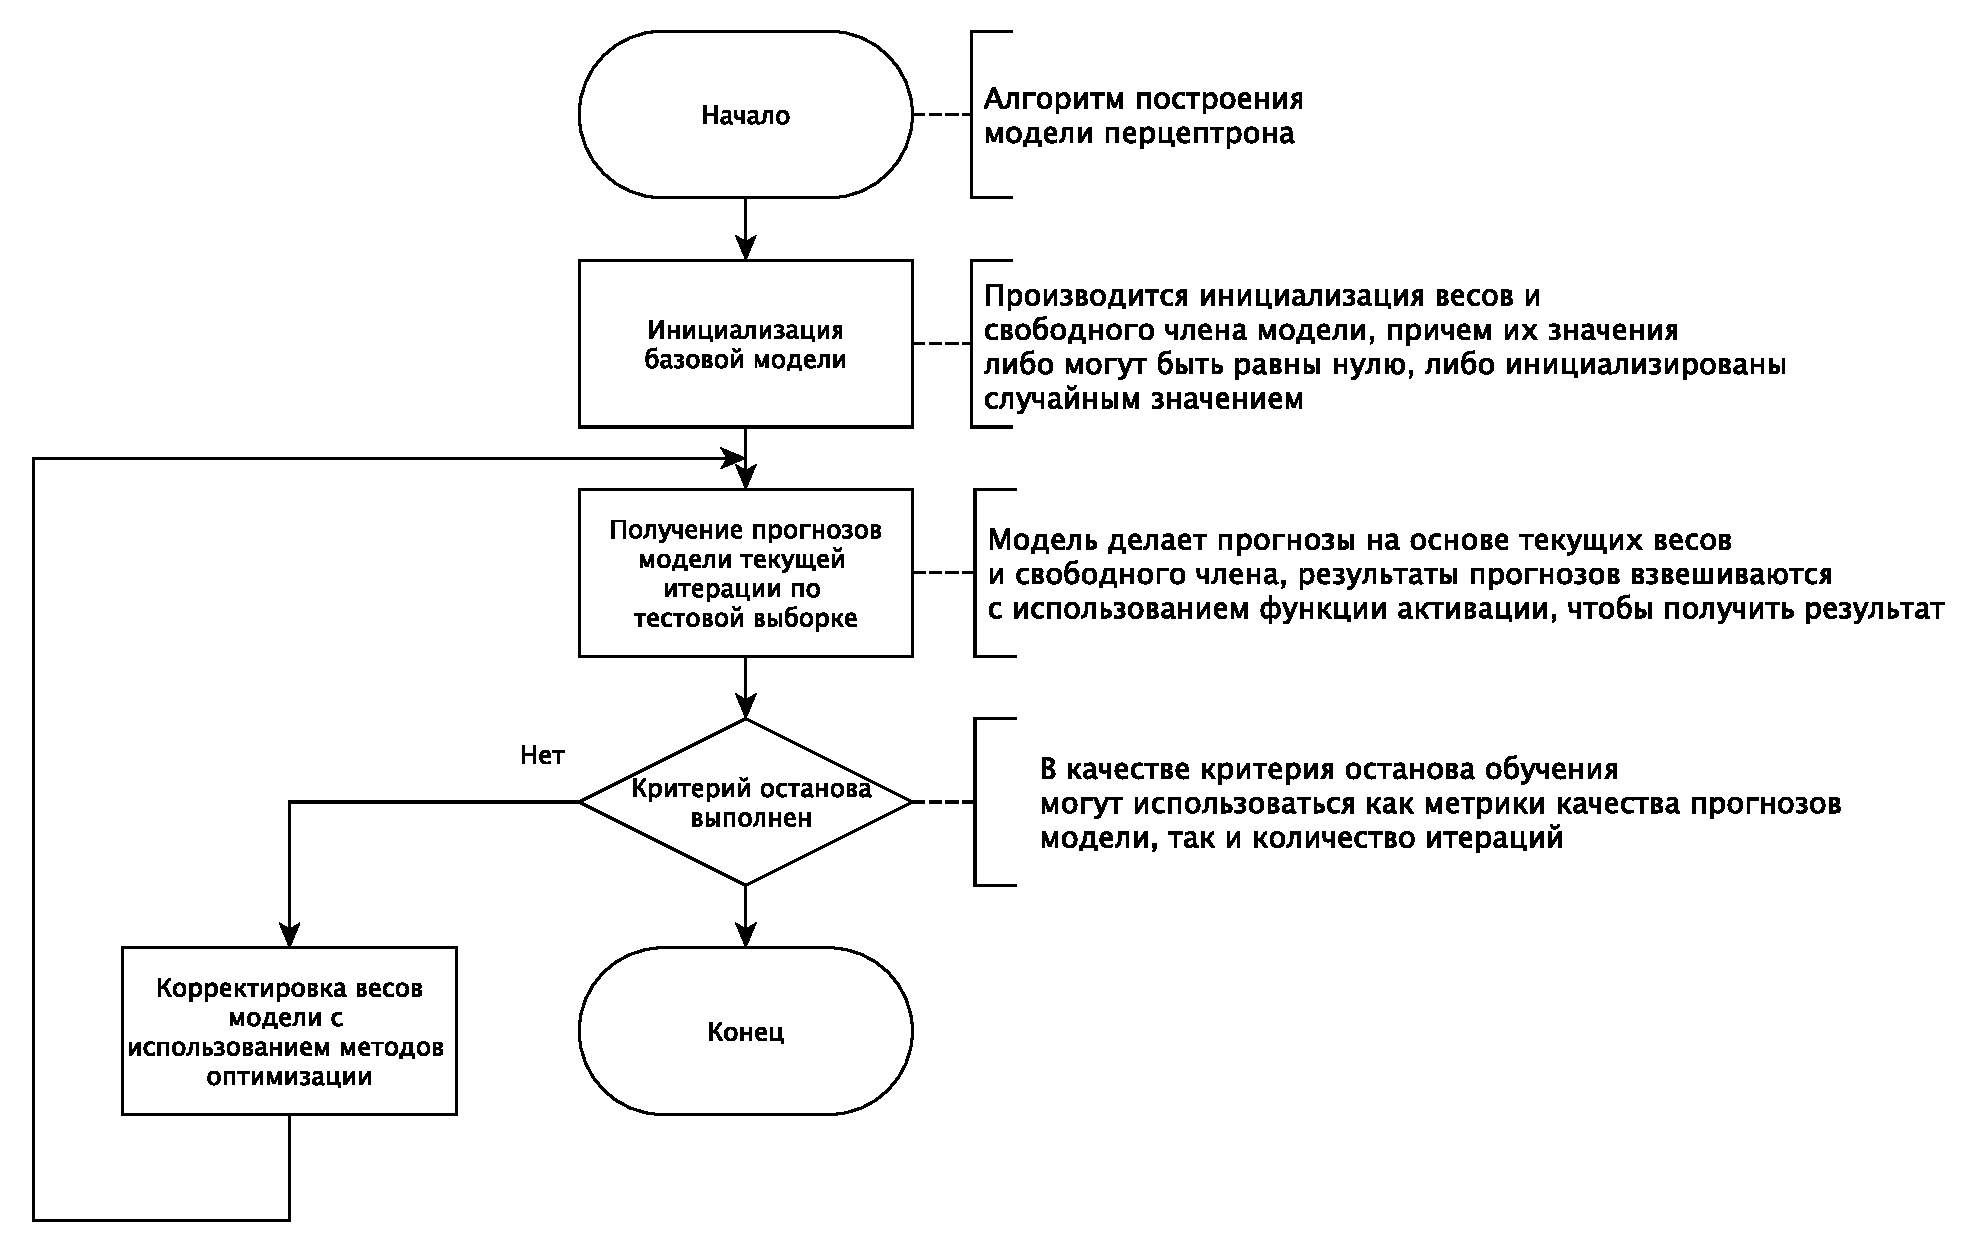
\includegraphics[width=\textwidth]{inc/schemePerceptrone.pdf}
	\caption{ Схема алгоритма работы метода с использованием перцептрона. }
	\label{img:schemePerceptrone}
\end{figure}

\subsection{Алгоритмы векторизации текстовых сообщений}

Классификация текстовых сообщений может производится с использованием вычленения ключевых слов, либо с использованием векторного представления данных.
Первый подход является наиболее простым, но к его недостаткам относят необходимость участия экспертов в создании словарей для описания каждого классифицируемого класса сообщений, кроме того для получения приемлемых результатов требуется, чтобы классы сообщений мало пересекались по словарному набору~\cite{vectorizations}.
Второй подход в классификации является более сложным, в нём могут использоваться различные модели векторизации для дальнейшей обработки текстовой информации.
В качестве задействованной здесь может выступать модель текста ``мешок слов''~\cite{bagOfWords} с его расширением для частотных характеристик встречаемости слов в сообщениях TF-IDF~\cite{tfIdf}.
Метод базируется на создании векторов сообщений с учетом весов встречаемости каждого слова, как в самом сообщении, так и во всех сообщениях выборки.
Его использование при построении классификатора значительно повышает точность классификации в некотором наборе задач~\cite{vectorizations}.

Кроме того, в качестве способа представления могут быть задействованы векторизации вида word embeddings.
В качестве основного механизма они задействуют модель word2vec~\cite{word2vec}, которая представляет собой нейронную сеть, ставящую подаваемому на вход слову в соответствие выходной вектор заданной длины.
Обучение нейронной сети производится таким образом, чтобы получить близкие в пространстве векторы для слов, встречающихся в одинаковых контекстах.
Таким образом, слова близкие по значению, либо употребляющиеся совместно, будут иметь близкие векторы в пространстве.
Существенным недостатком данного метода заключается в необходимости обучения нейронной сети на значительном корпусе текстов, что является ресурсозатратной задачей.
Эта проблема нивелируется существованием предобученных моделей.
Также к недостаткам относят невозможность представления слова, которого не было в обучающем корпусе.~\cite{vectorizations}

К векторизации word ebeddings также относят и проект ELMo \cite{elmo}. Данная модель обладает преимуществами word2vec и дополняет их возможностью формирования одного вектор на все сообщения, а также получения вектора для неизвестного слова путем его разложения на отдельные слоги и буквы.
В основе метода лежит многослойная нейронная сеть, которая на первом слое получает векторы для букв, а затем слои для работы со словами в составе всего сообщения.
В качестве вектора используются веса последнего слоя сети. Для данного подхода также существуют предобученные модели для многих языков, что значительно упрощает его использование.~\cite{vectorizations}

BERT \cite{bert} -- языковая модель, применяющаяся для анализа текста. Ее применение для построения классификатора требует обучения модели с кодированием отдельным слоем нейронной сети, что не дает возможность использовать данную технологию только для векторизации.
В отличие от прежних классических языковых моделей, BERT обучает контекстно-зависимые представления, причем он учитывает двусторонний контекст, что помогает модели лучше понимать смысл многозначных слов.~\cite{vectorizations}

Для векторизации собранных текстовых сообщений будут задействованы алгоритм ``мешок слов'' и языковая модель BERT.
Схемы работы выбранных алгоритмов представлены на рисунках \ref{img:schemeBagOfWords} и \ref{img:schemeBert} соответственно.
Алгоритм TF-IDF не входит в рассмотрение в силу того, что он является модернизацией алгоритма ``мешок слов''. 
Модели word2vec и ELMo также не попадают в рассмотрение в связи с тем, что данная работа первично имеет цель определить наиболее подходящий для решения задачи алгоритм машинного обучения.

\begin{figure}[H]
	\centering
	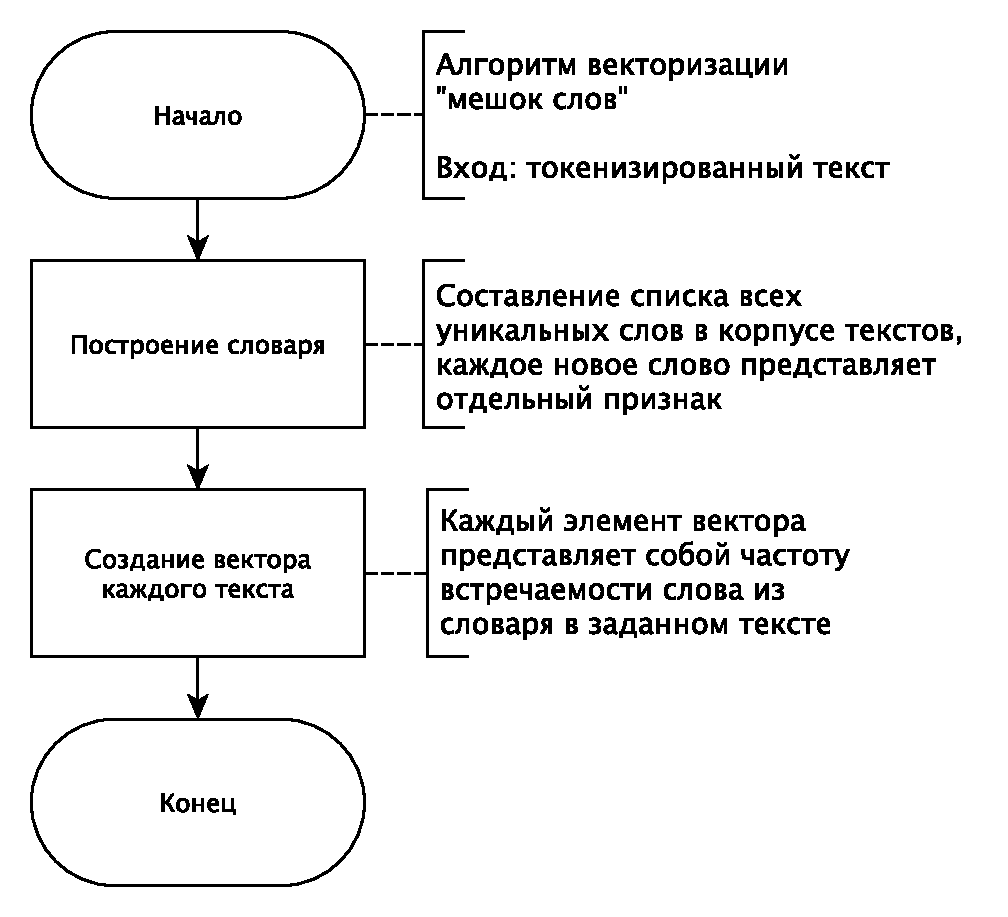
\includegraphics[width=0.5\textwidth]{inc/schemeBagOfWords.pdf}
	\caption{ Схема работы алгоритма ``мешок слов''. }
	\label{img:schemeBagOfWords}
\end{figure}

\begin{figure}[H]
	\centering
	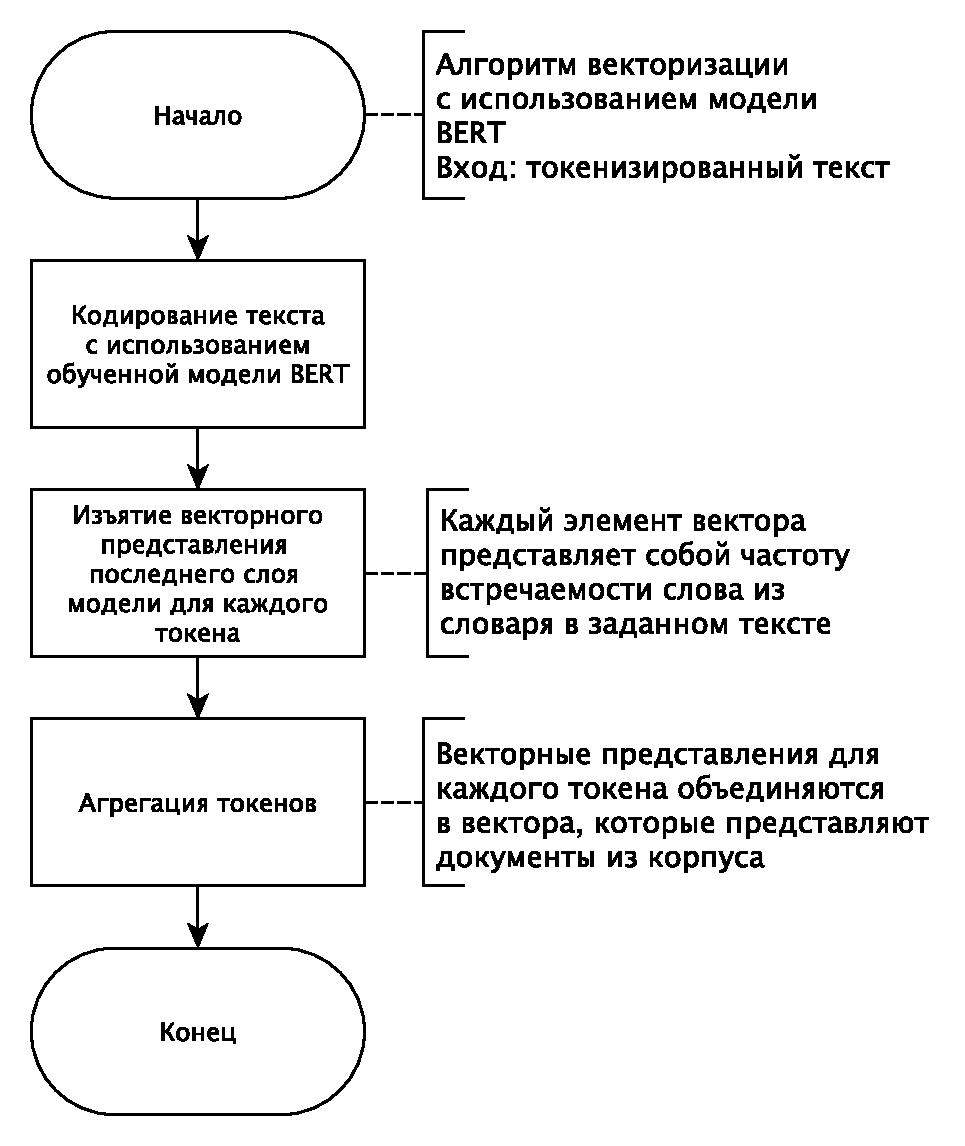
\includegraphics[width=0.4\textwidth]{inc/schemeBert.pdf}
	\caption{ Схема алгоритма векторизации с использованием модели BERT. }
	\label{img:schemeBert}
\end{figure}

\subsubsection*{Вывод}

Был описан метод распознавания суицидальных паттернов поведения человека по текстовым сообщениям, а также формат и метод сбора задействованных в нем данных. 
Определено, что в качестве средства сбора данных будет использоваться бот в мессенджере Telegram. Рассмотрены доступные средства реализации ботов в выбранном мессенджере.

Приведена диаграмма вариантов использования. Для системы было определено три действующих лица: пользователь, рекомендатор и анализатор. 
Приведена IDEF0 диаграмма, декомпозирована главная задача метода -- распознавание суицидального сообщения. 
Диаграмма ``сущность-связь'' в нотации Чена позволила на абстрактном уровне описать систему распознавания. 

Был определен перечень задействованных методов машинного обучения, который включил в себя: градиентный бустинг, метод случайного леса, метод опорных векторов, метод K-ближайших соседей, логистическая регрессия и перцептрон. В качестве методов векторизации выбраны: алгоритм ``мешок слов'' и языковая модель BERT.



\pagebreak